\documentclass[review]{elsarticle}
\usepackage{lineno,hyperref}
\usepackage{tikz, pgf, graphicx,import}
\usetikzlibrary{shapes.geometric, arrows,positioning,matrix,calc,intersections}
\usepackage{amsmath,booktabs,caption,subcaption}
\usepackage{booktabs, multicol,multirow, makecell, amsmath,afterpage}
\usepackage{tikz,tabularx, adjustbox}

\modulolinenumbers[5]
\journal{Journal of \LaTeX\ Templates}

%%%%%%%%%%%%%%%%%%%%%%%
%% Elsevier bibliography styles
%%%%%%%%%%%%%%%%%%%%%%%
%% To change the style, put a % in front of the second line of the current style and
%% remove the % from the second line of the style you would like to use.
%%%%%%%%%%%%%%%%%%%%%%%
%% Numbered
%\bibliographystyle{model1-num-names}

%% Numbered without titles
%\bibliographystyle{model1a-num-names}

%% Harvard
%\bibliographystyle{model2-names.bst}\biboptions{authoryear}

%% Vancouver numbered
%\usepackage{numcompress}\bibliographystyle{model3-num-names}

%% Vancouver name/year
%\usepackage{numcompress}\bibliographystyle{model4-names}\biboptions{authoryear}

%% APA style
%\bibliographystyle{model5-names}\biboptions{authoryear}

%% AMA style
%\usepackage{numcompress}\bibliographystyle{model6-num-names}

%% `Elsevier LaTeX' style
%\bibliographystyle{elsarticle-num}
%%%%%%%%%%%%%%%%%%%%%%%

\begin{document}

\begin{frontmatter}

\title{An approximation method of strength ratio calculation of laminated compoiste material based on evolutionary artificial neural network}
\tnotetext[mytitlenote]{Based on Evolving Artificial Neural Networks}

%% Group authors per affiliation:
%\author{}
%\address{}

%% or include affiliations in footnotes:

%\cortext[mycorrespondingauthor]{Corresponding author}
%\ead{support@elsevier.com}

%\address[mymainaddress]{}
%\address[mysecondaryaddress]{}

\begin{abstract}
Traditionally, classic lamination theory is widely used to compute
properties of composite materials under in-plane and out-of-plane loading from
a knowledge of the material properties of the individual layers and the
laminate geometry. In this study, a systematic procedure is proposed to design
an artificial neural network for a practical engineering problem, which is
applied to calculate the strength ratio of a laminated composite material under
in-plane loading, in which the genetic algorithm is proposed to optimize the search
process at four different levels: the architecture, parameters, connections of
the neural network, and active functions. 

\end{abstract}

\begin{keyword}
Classic Lamination Theory\sep Genetic Algorithm \sep Artificial neural network
\sep Optimization
\end{keyword}

\end{frontmatter}


%\linenumbers

\section{Introduction}
Fiber-reinforced composite materials have been widely used in a variety of
applications, which include electronic packaging, sports equipment,
homebuilding, medical prosthetic devices, high-performance military
structures, etc. because they offer improved mechanical stiffness, strength,
and low specific gravity of fibers over conventional materials.  The stacking
sequence, ply thickness, and fiber orientation of composite laminates give the
designer an additional ’degree of freedom’ to tailor the design with respect to
strength or stiffness. CLT and failure theory, e.g., Tsai-Wu failure criteria,
is usually taken to predict the behavior of a laminate from a knowledge of the
composite laminate properties of the individual layers and the laminate
geometry.

However, the use of CLT needs intensive computation which takes an analytical
method to solve the problem, since it involves massive matrix multiplication
and integration calculation. Techniques of function approximation can
accelerate the calculation process and reduce the computation cost.  Artificial
neural network(ANN), heavily inspired by biology and psychology, is a reliable
tool instead of a complicated mathematical model. ANN has been widely used to
solve various practical engineering problems in applications, such as pattern
recognition, nonlinear regression, data mining, clustering,  prediction, etc.
Evolutionary artificial neural networks(EANNs) is a special class of
artificial neural networks, in which evolutionary algorithms are
introduced to design the topology of an ANN, and can be used at four different
levels: connection weights, architectures, input features, and learning rules.
It is shown that the combinations of ANN's and EA's can significantly improve
the performance of intelligent systems than that rely's on ANN's or
evolutionary algorithms alone.

The rest of this paper is organized as the following: section II introduces the
CLT and the failure criteria, which is used to check whether the composite
material fails or not in the present study; section III covers the design of
artificial neural network for a function approximation; section IV reviews the
use of the genetic algorithm in the design of neural network architecture, and
the techniques of parameters optimization during the training process; section
V presents the result of the numerical experiments in different cases; in the
conclusion part, we present and discuss the experiment results.





\input{a1_introduction_part2_composite}
\section{Evolutionary Artificial Neural Network}
\subsection{General neural network}
In this paper, the feedforward ANN is adopted in the current
study, since it is straightforward and simple to code. For function
approximation through an ANN, Cybenko demonstrated that a two-layer perceptron
can form an arbitrarily close approximation to any continuous nonlinear
mapping\cite{cybenko1989approximation}. Therefore, a two-layer feedforward ANN
is proposed in the present study. Fig.\ref{fig:gnn} shows a general framework for a
two-layer NN, in which the number of nodes in the hidden layer and the
connection with inputs, are critical in the design of an ANN. For nodes in the
hidden layer, we can think of them as feature extractors or detectors.
Therefore, nodes within it should partially be connected with the inputs of an ANN,
since the unnecessary connections would increase the model's complicacy, which
will reduce an ANN’s performance. Because we treat the nodes in the hidden layer
as feature extractors, so the number of nodes in this layer should be less than
the number of inputs. For the nodes in the last layer, every node should be
fully connected with nodes in the previous layer, since we think of the nodes
in the hidden layer as features. The rest, which affects a NN’s performance,
are transfer function, and ANN's training method. In the following section, we
denote the $i$th node in the input layer, and the hidden layer, as $i_i$, and $h_i$,
recpectively.

\begin{figure}[!t]
	\centering
	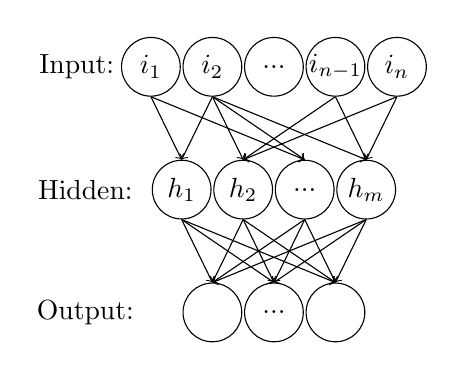
\begin{tikzpicture}
		[ plain/.style={ draw=none, fill=none, }, remember picture, net/.style={ matrix of nodes, nodes={ draw, circle,
			inner sep=7.5pt
			},
		  nodes in empty cells,
		  column sep=-10.5pt,
		  row sep=0.8cm
		  }
		]
	%\draw[help lines] (-3cm,-6cm) grid (6cm,3cm);
	\matrix[net] (mat)
		{
				  & |[plain]| &           & |[plain]|  &           & |[plain]| &           &  |[plain]|      &               \\
		|[plain]| &           & |[plain]| &            & |[plain]| &           & |[plain]| &                 & |[plain]|     \\ 
		|[plain]| & |[plain]| &           & |[plain]|  &           & |[plain]| & 	  	   &  |[plain]|      & |[plain]|     \\ 
	  };

	  \node at ($(mat-1-1.west)+(-16pt,0)$) {Input: };
	  \node at ($(mat-2-2.west)+(-24pt,0)$) {Hidden:};
	  \node at ($(mat-3-2.west)+(-24pt,0)$) {Output:};
	  \node at (mat-1-1.base) {$i_1$};
	  \node at (mat-1-3.base) {$i_2$};
	  \node at (mat-1-5.base) {...};
	  \node at (mat-1-7.base) {$i_{n-1}$};
	  \node at (mat-1-9.base) {$i_{n}$};
	  \node at (mat-2-2.base) {$h_1$};
	  \node at (mat-2-4.base) {$h_2$};
	  \node at (mat-2-6.base) {$...$};
	  \node at (mat-2-8.base) {$h_{m}$};
	  \node at (mat-3-5.base) {$...$};

		 \foreach \a in {1,3}{
			\foreach \b in {2,6}{
				\draw[->] (mat-1-\a.south) -- (mat-2-\b.north);
			 }
		  }
		 \foreach \a in {3,7,9}{
			\foreach \b in {4,8}{
				\draw[->] (mat-1-\a.south) -- (mat-2-\b.north);
			 }
		  }

		 \foreach \c in {2,4,6,8}{
			\foreach \d in {3,5,7}{
				\draw[->] (mat-2-\c.south) -- (mat-3-\d.north);
			}
	 }
\end{tikzpicture}
\caption{Network diagram for the two-layer neural network. The input, hidden,
		and output variables are represented by nodes, and the weight parameters are
		represented by links between the nodes. Arrows denote the direction of
		information flow through the network during forward propagation.}
\label{fig:gnn}
\end{figure}






\subsection{Transfer function}

The transfer function is one of the critical parts of an ANN. Liu
\cite{liu1996evolutionary} et al. claims that the performance of NNs with
different transfer functions is different, even if they have the same
architecture.  A generalized transfer function can be written as

\begin{equation}
	y_i = f_i(\sum_{j=1}^n{w_{ij}x_j - \theta})
\end{equation}

where $y_i$ is the output of the node $i$, $x_j$ is the $j$th input to the
node, and $w_{ij}$ is the connection weight between adjacent nodes $i$ and $j$.
Tab. \ref{tab:transfer_function} display the most widely adopted transfer
functions in the design of an ANN, which is used for the current study.

\begin{table*}[!t]
\centering
\caption{Different Activation Functions}
\label{tab:active_function}
\begin{adjustbox}{width=0.9\textwidth}
\label{tab:transfer_function}
	\begin{tabular}{lllcc}
			\toprule
			Type & Description  & Formula & Range              & Encoding\\
			\midrule
			Linear   & The output is proportional to the input & $f(x)=cx$                  &  $(-\infty, +\infty)$ & 00\\
			Sigmoid  & A family of S-shaped functions          & $f(x)=\frac{1}{1+e^{-cx}}$ & $(0, 1)$              & 01\\
			ReLU     & A piece-wise function                   & $f(x)= max{0,x}$           & $(0, +\infty)$        & 10\\
			Softplus & A family of S-shaped functions          & $f(x) = ln(1+e^x)$         & $(0, +\infty)$        & 11\\
			\bottomrule
	\end{tabular}
\end{adjustbox}
\end{table*}


\subsection{Weights learning}
The weight training in an ANN is to minimize the error function, such as the
most widely used mean square error function, which calculates the difference
between the desired and the prediction output values averaged overall examples.
Gradient descent algorithm is widely adopted to reduce the value of an error
function, which has been successfully applied in many practical areas. However,
this class of algorithms is plagued by the possible existence of local minima
or ”flat spots” and ”the curse of dimensionality.” One method to overcome this
problem is to adopt a genetic algorithm(GA)


\section{Methodology}
\subsection{Objective function}
The optimization problem can be formulated by searching the optimal stacking
sequence of composite laminate.  There are two design variables here, the angles
in the laminate, and the number of layers that each fiber orientation has. The
objective function is formulated as

\begin{equation}
	\begin{split}
    	F  &= 2t_0 \sum_{k=1}^n n_k  \textstyle{,}\\
    	   &SF_{MS} \geq 1 \textstyle{,} \\
    	   &SF_{TW} \geq 1 \textstyle{.}
	\end{split} 
\end{equation}

The first term represents the total thickness of the composite laminates, $t_0$
is the ply thickness; $n_k$ is the number of plies in the kth lamina, in which
the fiber orientation is $\theta_k$. The constraints here are two safety
factors should not less than 1, which means  $SF_{MS} \geq 1$, and $SF_{TW} \geq
1$, respectively.

\subsection{Encoding}
Due to the simplicity and efficiency of float representation, this encoding
method is implemented to represent a possible solution. As shown in Figure \ref{GA:operator}
 (a), these two chromsomes represent a $[+8_{7}/-9_{2}]_s$
carbon T300/5308 laminated composite, and $[+19_{4}/-36_{6}]_s$, respectively.
Becasue the laminate adopted in this paper is symmetric to its mid-plane, so
only half needs to be encoded.

\subsection{Selection}
The purpose of the selection operator is to choose mating pool to produce
alternative solutions of better fitness. Traditional methods of selecting
strategies only take the fitness of individuals into account, however, due to 
the existence of constraint, various selection schemes are implemented to
select the mating set. Based on different selection schemes, the parents of
next generation can be divided into  three groups: proper groups, active groups,
and potential groups according to different selecting methods. 

Proper parents mean in which individual fullfills the constraints, which are
chosen by the individual's fitness, individuals with better fitness are more
likely to be chosen if they fit the constraint; active group means that
individual within this group is supposed to always exist in the parents during the GA, which
are selected by fitness, ignoring the constraint; The individuals from the active
group may not correspond to feasible solutions, but their existence enriches the
variety of the gene clips.  Potential group means that individuals are likely to turn
into proper individual after a couple of generations, and potential individuals
are chosen by constraint function, the more the individual fulfills the
constraint, the more possibility it will be selected.

\subsection{Crossover}
The crossover operator happens among these three groups. the child of two proper
groups is more likely to be a proper individual which can be used to obtain an
alternative feasible solution. the child of an active individual and a potential
individual can significantly change the gene of an active individual's chromosome,
which makes the individual evolve toward a new direction. The offspring of two
active individuals are more likely to be an active individual, which can maintain
the active group.  The figure.\ref{GA:operator} (b) shows two children $O_1$
and $O_2$ from two parents $P_1$ and $P_2$, each angle $C_a$ and its length 
$C_l$ of a child are obtained by the following formula
\begin{align} 
	\begin{cases}
	C_a &= (P1_a + P2_a)/2 \\
	C_l &= (P1_l + P2_l)/2 
\end{cases} \textstyle{.}
\end{align}
\begin{table}[tb]
\caption{Comparison of the carbon/epoxy, graphite/epoxy, and glass/epoxy properties}
\centering
\begin{adjustbox}{width=0.5\textwidth}
\label{tab:mat}
\begin{tabular}{lccccc}
\toprule
Property								   & Symbol				  & Unit  &  Carbon/Epoxy&  Graphite/Epoxy  &  Glass/Epoxy   \\
\midrule
Longitudinal elastic modulus			   & $E_1$				  & GPa   &  116.6       &  181             &  38.6           \\
Traverse elastic modulus				   & $E_2$				  & GPa   &  7.67        &  10.3            &  8.27           \\
Major Poisson's ratio					   & $v_{12}$			  &       &  0.27        &  0.28            &  0.26           \\
Shear modulus							   & $G_{12}$			  & GPa   &  4.17        &  7.17            &  4.14           \\
Ultimate longitudinal tensile strength     & $(\sigma_1^T)_{ult}$ & MP    &  2062        &  1500            &  1062            \\
Ultimate longitudinal compressive strength & $(\sigma_1^C)_{ult}$ & MP    &  1701        &  1500            &  610             \\
Ultimate transverse tensile strength       & $(\sigma_2^T)_{ult}$ & MPa   &  70          &  40              &  31              \\
Ultimate transverse compressive strength   & $(\sigma_2^C)_{ult}$ & MPa   &  240         &  246             &  118              \\
Ultimate in-plane shear strength           & $(\tau_{12})_{ult}$  & MPa   &  105         &  68              &  72               \\
Density                                    & $\rho$               & $g/cm^3$ &  1.605    &  1.590           &  1.903               \\
Cost                                       &                      &       &  8           &  2.5             &  1               \\
\bottomrule
\end{tabular}
\end{adjustbox}
\end{table}

\subsection{Mutation}
A mutation direction is imposed on the mutation operator which to make sure the
individual evolving toward the right direction. The mutation direction, denoted
by $md$, is an n dimensional vector corresponding to the number of constraints, it
is decided by the constraint thresholds $CT_i$ and the current individual's
constraint value, denoted as $CV_i$,  The mutation vector can be obtained by the
following formula

\resizebox{.9\linewidth}{!}{
	$\text{md} = [CT_1, \cdots, CT_{n-1}, CT_n] -  [CV_0, \cdots, CV_{n-1}, CV_n] \textstyle{.}$

}

During this operator, the mutation procedure is consist of two phases: the length
mutation of the chromosome, and the angle mutation of the chromosome.  Because the
chromosome's length is positively correlated with the individual's fitness, the
coefficient of length mutation denoted by $C_l$, if $\sum_{i=1}^{N}{CT_i}$ great
than $\sum_{i=1}^{N}{CV_i}$ , the mutation length is restricted to the range
$[0,(C_l \sum_{i=1}^{N}{(CT_i-CV_i)})/N]$, which means increase the chromosome's
length; Assuming a $[+13_6/-27_4]_s$ T300/5308 carbon/epoxy composite
laminate under the loading $N_{x} = N_{y} = 10$ MPa m, it's property as shown
in table \ref{tab:T300/5308}. According to CLT and
failure theory, the two safety factors $SF_{MS}$ and $SF_{TW}$ are  0.0539, and
0.0540, respectively. So the mutation vector and is $[0.9461,0.9460]$, assuming
the length mutation coefficient is 20, so the mutation range is from 0 to 18. A
random number is generated from the range $[0, 18]$, supposing the outcome is
13, then a length generator is used to a list, the its sum is 13, suppose the
list is [5, 8], the laminate after mutation is $[13_{11}/-27_{12}]_s$.

If the $\sum_{i=1}^{N}{CT_i}$ less than $\sum_{i=1}^{N}{CV_i}$, the
mutation length is restricted to the range $([\sum_{i=1}^{N}{CT_i-CV_i})/N,0]$,
which means the individual's fitness exceeds the threshold value, and decrease
the chromsome's length.  Assuming a $[+33_{35}/-29_{26}]_s$ T300/5308 laminate
is under loading $N_{x}=10$ MPa, and $N_{y}=5$ MPa, then, it's $SF_{MS}$
constraint and $SF_{TW}$ values are  1.0912, 1.0747, respectively.
because the length mutation is 20, so the mutation range is from -2 to 0. This
would decrease the chromosome's length. 
\begin{align}
	\text{LM} = 
	\begin{cases}
		\resizebox{.35\textwidth}{!}{$[0,(C_l \sum_{i=1}^{N}{(CT_i-CV_i)})/N], \text{ if }  \sum_{i=1}^{N}{CT_i} > 
		\sum_{i=1}^{N}{CV_i}$}\\
		\resizebox{.35\textwidth}{!}{$[(C_l \sum_{i=1}^{N}{(CT_i-CV_i)})/N,0], \text{ if }  \sum_{i=1}^{N}{CT_i} < 
		\sum_{i=1}^{N}{CV_i}$}\\
	\end{cases} 
\end{align}

The relationship between the angles in the composite laminate and the
chromosome's fitness is unclear, so the mutation direction of chromosome's angle
is random. The coefficient angle mutation is $C_a$, the angle mutation range is
$[0,C_a \sum_{i=1}^{N}{(|CT_i-CV_i|)}]$ or $[C_a
\sum_{i=1}^{N}{(-|CT_i-CV_i|)},0]$. It is can be written as

\begin{align}
	\text{P(AM)} =  
	\begin{cases}
		0.5, \text{ AM = }[0,C_a \sum_{i=1}^{N}{(|CT_i-CV_i|)}] \\ 
	    0.5, \text{ AM = }[C_a \sum_{i=1}^{N}{(-|CT_i-CV_i|)},0]
	\end{cases} \textstyle{.}
\end{align}

\section{Experiment}
In the previous section we present the details of our strategies for designing an ANN. In
this section, we describe the details of praparation of training set, and validation set.
\subsection{Dataset Preparation}
For compoiste material, it is impossible to obtain massive training data from
practical scenerio.  Therefore, we use classical lamination theory and failure
theory to prepare the training dataset, which follows a two-step procedure to
calculate the strength ratio: first, evaluate the stress and strain according
to classic lamination theory; second, substitue them into the corresponding
equation to get the strength ratio. We repeat this procedure to yield 14000
points uniformly distributed over the domain space.

The range of in-plane loading is from 0 to 120; the range of fiber orientation $\theta$ is from
-90 to 90; ply thickness $t$ is 1.27mm, number of plies range $N$ is from 4 to 120;
Three different material is used in this experiment, as shown in table \ref{tab:mat}.
Figure \ref{tab:traing-data} shows part of the training data.

In order to speeds up the learning and accerlate convergence, the input
atttributes of the dataset are rescaled to between 0 and 1.0 by a linear function.



\begin{table}[!t]	
\centering
\caption{Examples of the training data}
\label{tab:traing-data}
\begin{adjustbox}{width=0.5\textwidth}
	\begin{tabular}{cccc|cc}
		\toprule
		\multicolumn{4}{c}{\textbf{Input}} &  \multicolumn{2}{c}{\textbf{Output}} \\
		\midrule
		Load  &  \makecell{Laminate \\ Structure }  & \makecell{Material \\ Property} & \makecell{Failure \\  Property}  & MS & Tsai-Wu \\
		\midrule

		-70,-10,-40,  & 90,-90,4,1.27, & 38.6,8.27,0.26,4.14,  & 1062.0,610.0,31,118,72,  & 0.0102, & 0.0086 \\
		-10,10,0,     & -86,86,80,1.27,& 181.0,10.3,0.28,7.17, & 1500.0,1500.0,40,246,68, & 0.4026, & 2.5120 \\
		-70,-50,80,   & -38,38,4,1.27, & 116.6,7.67,0.27,4.173,& 2062.0,1701.0,70,240,105,& 0.0080, & 0.0325 \\
		-70,80,-40,   & 90,-90,48,1.27,& 38.6,8.27,0.26,4.14,  & 1062.0,610.0,31,118,72,  & 0.0218, & 0.1028 \\
		-20,-30,0,    & -86,86,60,1.27,& 181.0,10.3,0.28,7.17, & 1500.0,1500.0,40,246,68, & 0.6481, & 0.9512 \\
		0,-40,0,      & 74,-74,168,1.27,& 181.0,10.3,0.28,7.17,& 1500.0,1500.0,40,246,68, & 1.3110, & 3.9619 \\
		\bottomrule
		\end{tabular}
\end{adjustbox}
\end{table}


The ANN training procedure is carried out by optimising the multinomial
logistic regression objective using mini-batch gradient descent\cite{lecun1989backpropagation} with momentum. the batch size is set to 1000,
momentum to 0.9. the learning rate is set to $10^{-2}$.


\section{Result and Discussion}
We have conducted experiment by the use of the generated data set. This data
set is randomly partitoned into a training set and a test.

Figure \ref{fig:train-process} shows five ANNs with different topologies, quite
different results have been observed when different architectures are adopted.
It is clear that architecture whose mean of average difference is less than the
rest.


\begin{figure}
	\centering
	\def\svgwidth{\columnwidth}
	\import{fig/}{pre_train.pdf_tex}
	\label{fig:train-process}
\end{figure}

Table \ref{tab:simu} shows part of the valudation.
\begin{table}[!tb]
	\centering
	\caption{ANN predictions of the Tsai-wu and MS strength ratio with the
	numberical results obtained by CLT.}
	\label{tab:simu}
	\begin{adjustbox}{width=0.5\textwidth}
	\begin{tabular}{cccc|cc|cc}
		\toprule
		\multicolumn{4}{c}{\textbf{Input}} &  \multicolumn{4}{c}{\textbf{Output}} \\
		\midrule
		Load  &  \makecell{Laminate \\ Structure }  & \makecell{Material \\ Property} & \makecell{Failure \\  Property}  &
		\multicolumn{2}{c}{ \makecell {CLT \\MS  Tsai-Wu}} & \multicolumn{2}{c}{ \makecell {ANN \\MS  Tsai-Wu}}\\
		\midrule
		-10,40,20  &  26,-26,168,1.27 & 116.6,7.67,0.27,4.17 & 2062.0,1701.0,70,240,105 & 0.342 & 0.476 & 0.351 & 0.492 \\
		20,-70,-30 &  10,-10,196,1.27 & 181.0,10.3,0.28,7.17 & 1500.0,1500.0,40,246,68  & 0.653 & 0.489 & 0.612 & 0.445 \\ 
		60,-20,0   &  82 -82,128,1.27 & 181.0,10.3,0.28,7.17 & 1500.0,1500.0,40,246,68  & 1.663 & 0.112 & 1.673 & 0.189 \\
		\bottomrule
	\end{tabular}
	\end{adjustbox}
\end{table}



\begin{figure}
	\centering
	\def\svgwidth{\columnwidth}
	\import{fig/}{post_train.pdf_tex}
	\label{fig:final_train}
\end{figure}


Comparing the strength ratio outputs based on CLT and ANN from
Tab.\ref{tab:simu}, we can see that the calculation of strength ratio can be
achieved using a two-layer neural network, without the intensive computation of
matrix multiplication.





\section{Conclusion}
In this paper, an evolutionary artificial neural network model was developed to
predict the strength ratio of laminated composite material under in-plane
loading. We review the use of genetic algorithms and artificial neural networks
as an alternative approach for calculating the strength ratio of an angle ply
laminate under in-plane loading. Traditionally, it is obtained through CLT and
corresponding failure criteria, such as Maximum Stress theory and Tsai-Wu
failure theory.

The main contribution of this work is as follows: 1) propose a two-layer diagram
model for designing a sophisticated neural network in simulating the calculation
of strength ratio, and use a genetic algorithm to explore the search space. 2)
suggest an efficient method to compute the strength ratio instead of adopting
the two-step procedure based on classical lamination theory and related failure
criteria. Compared with experimentally obtained data, it is demonstrated that
ANN is an efficient and simple tool to compute the strength ratio, instead of
the complex analytical mathematical model. Our findings underline the practical
applicability of ANN on the analysis of composite material.

There are more improvements we can make over the search strategy and application
in the area of laminated composite material. The future work is to develop a
more sophisticated ANN, which not only can predict the properties for angle ply
laminate, but also the other type of laminated composite material.


\section*{Acknowledgment}
The work has partly been supported by China Scholarship
Council(CSC) under grant no. 201806630112


\bibliographystyle{plain}
\bibliography{a5_reference}

\end{document}
